\documentclass[aspectratio=1610]{beamer}
\usetheme{lug}
\usepackage{xcolor}
\usepackage{fontspec}
\usepackage{minted}
\setminted{autogobble}
\usemintedstyle{lovelace}
\beamertemplatenavigationsymbolsempty
\setbeamercovered{dynamic}

\title{Readline Ninja Skills}
\author{Jack Rosenthal}
\date{2016-03-07 \\ 2018-03-08}

\begin{document}
\begin{frame}
    \maketitle
\end{frame}

\begin{frame}
    \frametitle{Readline}
    \begin{itemize}[<+->]
        \item A library for interactive line editing that your shell probably uses.
        \item Responsible for things like tab completion, history expansion,
            and all of those useful keystrokes
        \item Readline saves you keystrokes.
        \item Some readline things can make you look like a total ninja.
        \item Some readline things make you feel like a total ninja.
    \end{itemize}
\end{frame}

\section{Using Readline \& History}

\begin{frame}
    \frametitle{History}
    Readline can track your history, most shells let you use the
    \texttt{history} builtin to view your history.

    You can navigate your history using the up and down keys.
\end{frame}

\begin{frame}
    \frametitle{Tab completion}
    Most of us already know what this and would die without it.
\end{frame}

\begin{frame}
    \frametitle{Event Designators}
    \begin{itemize}[<+->]
        \item \texttt{!} - begin history expansion
        \item \texttt{!!} - refer to the last command
        \item \texttt{!$n$} - refer to the $n$-th command in history
        \item \texttt{!-$n$} - refer to the current command minus $n$
        \item \texttt{!\#} - refer to the current command you are typing
        \item \texttt{!$search$} - refer to the last commmand that starts with
            $search$
        \item[] \texttt{!?$search$?} - refer to the last command with $search$
            anywhere in the command
    \end{itemize}
    \pause[\thebeamerpauses]
    Examples:
    \begin{itemize}[<+->]
        \item \texttt{sudo !!} - run the last command with \texttt{sudo} in
            front
        \item \texttt{!grep} - run the last command you typed beginning with
            \texttt{grep}
    \end{itemize}
\end{frame}

\begin{frame}
    \frametitle{Word Designators}
    Often times you will want only part of a command, so you can use word
    designators to select which parts you want.\pause{} Follow an event designator with
    a colon (\texttt{:}) and then a word designator.
    \pause
    \begin{itemize}[<+->]
        \item \texttt{:$n$} - select argument $n$ (zero indexed)
        \item \texttt{:$n$-$m$} - select arguments $n$ through $m$
        \item \texttt{:\$} - select the last argument (think of a regex)
        \item \texttt{:*} - select all arguments, omitting the command name
            (equivalent to \texttt{:1-\$})
        \item[] \texttt{:\%} - select the argument that matches
                \texttt{?$search$?}
    \end{itemize}
    \pause[\thebeamerpauses]
    Examples:
    \begin{itemize}[<+->]
        \item \texttt{cd !!:1} - \texttt{cd} to the first argument of the last
            command.
        \item \texttt{vim !-2:\$} - edit the file that is the last argument of
            two commands ago
    \end{itemize}
\end{frame}

\begin{frame}
    \frametitle{Modifiers}
    \only<1-8>{
    Modifiers let you chop up the history expansion in ways that you like. You
    can chain any amount of modifiers that you would like onto your expansion.
    }
    \begin{itemize}
        \item<2-> \texttt{:r} - Chop off the extension of a filename
        \item<3-> \texttt{:h} - Remove the filename component, leaving only the
            directory (think of head)
        \item<4-> \texttt{:t} - Remove the directory component, leaving only the
            filename (think of tail)
        \item<5-> \texttt{:q} - Quote each of the arguments
        \item<6-> \texttt{:s/$search$/$replace$/} - \texttt{sed} style substitution
        \item<7-> \texttt{:gs/$search$/$replace$/} - \texttt{sed} style
            substitution, globally
        \item<8-> \texttt{:p} - print the history expansion, don't execute quite
            yet
    \end{itemize}
    \only<9->{
    Examples:
    \begin{itemize}
        \item<10-> \texttt{mv important.png !\#:1:r.gif} - rename
            \texttt{important.png} to \texttt{important.gif}
        \item<11-> \texttt{touch mydir/file.txt}
        \item<12-> \texttt{cd !\$:h}
    \end{itemize}
}
\end{frame}

\begin{frame}
    \frametitle{Abbreviations Allowed}
    \begin{itemize}[<+->]
        \item \texttt{!!:\ldots} can be shortened to \texttt{!:\ldots}
        \item The \texttt{:} can be removed from word designators where it is
            unambiguous. So \texttt{!\$} and \texttt{!*} are allowed.
        \item The trailing \texttt{/} in a substitution can be omitted if it is
            unambigous that the substitution has ended.
        \item The trailing \texttt{?} in a \texttt{!?$search$?} can be ommitted
            for the same reason.
        \item Any delimiter can be used in a substitution, so
            \texttt{!:sx$find$x$replace$x} is legal.
    \end{itemize}
\end{frame}

\begin{frame}
    \frametitle{Editing Modes}
    Readline provides editing modes similar to \texttt{vi} and \texttt{emacs}.
    Learn one and learn to love it. Most shells and programs have
    \texttt{emacs} as the default.
\end{frame}

\begin{frame}
    \frametitle{History Incremental Search}
    \texttt{<C-r>} (\texttt{vi: <Esc>/}) brings you to an search of your
    history. \texttt{<C-s>} will reverse the direction of your search (You may
    need to \texttt{stty -ixon}).
\end{frame}

\section{Readline Programming in C/C++}

\begin{frame}[fragile=singleslide]
    \frametitle{C/C++ Readline Library}
    \inputminted{c}{codesnip/readlineinclude.c}

    Allocates memory to read a line, reads it from standard input (displaying
    \mintinline{c}{prompt} as the prompt line). Returns the line you read. You
    really should \mintinline{c}{free} the memory it allocated.
\end{frame}

\begin{frame}[fragile]
    \frametitle{Using History Features}
    \begin{minted}{c}
        void using_history(void);
    \end{minted}
    Must be called before using history features.
    \pause

    \begin{minted}{c}
        int read_history(const char *filename);
        int write_history(const char *filename);
    \end{minted}
    For reading/writing saved history. Returns non-zero on failure and sets
    \mintinline{c}{errno}.
    \pause

    \begin{minted}{c}
        void add_history(const char *line);
    \end{minted}
    Add a line to the history.
    \pause

    \inputminted{c}{codesnip/historylist.c}
    List history.
\end{frame}

\begin{frame}[fragile]
    \frametitle{History Expansion (for free!)}
    \begin{minted}{c}
        int history_expand(char *string, char **output);
    \end{minted}

    Expand string, placing the result into output, a pointer to a string.  Returns:
    \begin{tabular}{l l}
        0 &    If no expansions took place \\
        1 &    If expansions did take place \\
        -1 &   If there was an error in expansion \\
        2 &    If the line should be displayed, but not executed (\texttt{:p}) \\
    \end{tabular}

    If an error occurred in expansion, then output contains a descriptive error
    message.
\end{frame}

\begin{frame}[fragile]{A Complete Example: 31-line UNIX shell}
    \tiny
    \inputminted[linenos]{c}{codesnip/progexample.c}
\end{frame}

\section{Readline Programming in Python}

\begin{frame}[fragile]{\texttt{import readline}}

    To use Readline from Python, type \texttt{import readline}, and the
    \texttt{input} function will magically become readlineifyed.

    \begin{minted}{python3}
        import sys
        import readline

        while True:
            try:
                cmd = input(">>> ")
            except KeyboardInterrupt:
                continue
            except EOFError:
                sys.exit(0)
            print(exec(cmd))
    \end{minted}
\end{frame}

\begin{frame}[fragile]{Tab Completion}
    The \texttt{readline} module provides an interface for you to add your own
    completer:

    \begin{minted}{python3}
        readline.set_completer(function)
    \end{minted}

    \mintinline{python3}{function} should be a function which takes two
    parameters:

    \begin{tabular}{l l}
        \texttt{text} & The current completion text \\
        \texttt{state} & \texttt{0}, \texttt{1}, \ldots \\
    \end{tabular}

    \pause

    Then, set your delimiters and completion keys:
    \begin{minted}{python3}
        readline.set_completer_delims(' ')
        readline.parse_and_bind("tab: complete")
    \end{minted}
\end{frame}

\begin{frame}[fragile]{Custom Completion in the Wild: \texttt{iels}}
    \fontsize{9pt}{10pt}\selectfont
    \begin{minted}[linenos]{python3}
        def completer(text, state):
            def gen():
                variables = reduce(set.union, map(dict.keys, els.vars), set())
                for s in '%', '$':
                    for v in variables:
                        if (s + v).startswith(text):
                            yield s + v
                for op in els.operators:
                    if op.startswith(text):
                        yield op
                for syntax in 'begin', 'end':
                    if syntax.startswith(text):
                        yield syntax

            if state == 0:
                completer.it = gen()

            try:
                return next(completer.it)
            except StopIteration:
                return None
    \end{minted}
\end{frame}

\begin{frame}{Alternatives to Readline for Python}
    While Readline is a well written piece of software, it feels a little bit
    out of place in Python, with the bindings reflective of the
    state-maintaining C code they talk to.

    Prompt Toolkit is a pure-Python alternative with fancy features:

    \begin{center}
        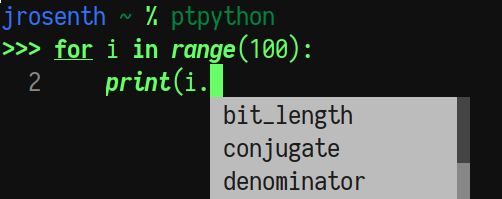
\includegraphics[width=0.8\textwidth]{graphics/ptpython.png}
    \end{center}
\end{frame}

\section{Further Resources}

\begin{frame}{More Info}
    \begin{enumerate}
        \item \texttt{man 3 readline}
        \item \texttt{man 3 history}
        \item \texttt{pydoc readline}
        \item RTFM: Read The \emph{Fine} Manual
    \end{enumerate}
\end{frame}

{
    \setbeamercolor{background canvas}{bg=csmblue}
\begin{frame}

    \begin{center}
        \Huge\headingfont
        \color{white}{Questions?}
    \end{center}

\end{frame}
}

\end{document}
